\documentclass{standalone}
\usepackage{tikz}
\usetikzlibrary{patterns}
\usetikzlibrary{positioning}
\usetikzlibrary{patterns, positioning}
\usetikzlibrary{shapes.misc}
\usepackage[outline]{contour}
\contourlength{1.5pt} 
\usetikzlibrary{calc}
        \usepackage{relsize}
        \tikzset{fontscale/.style = {font=\relsize{#1}}}

\begin{document}
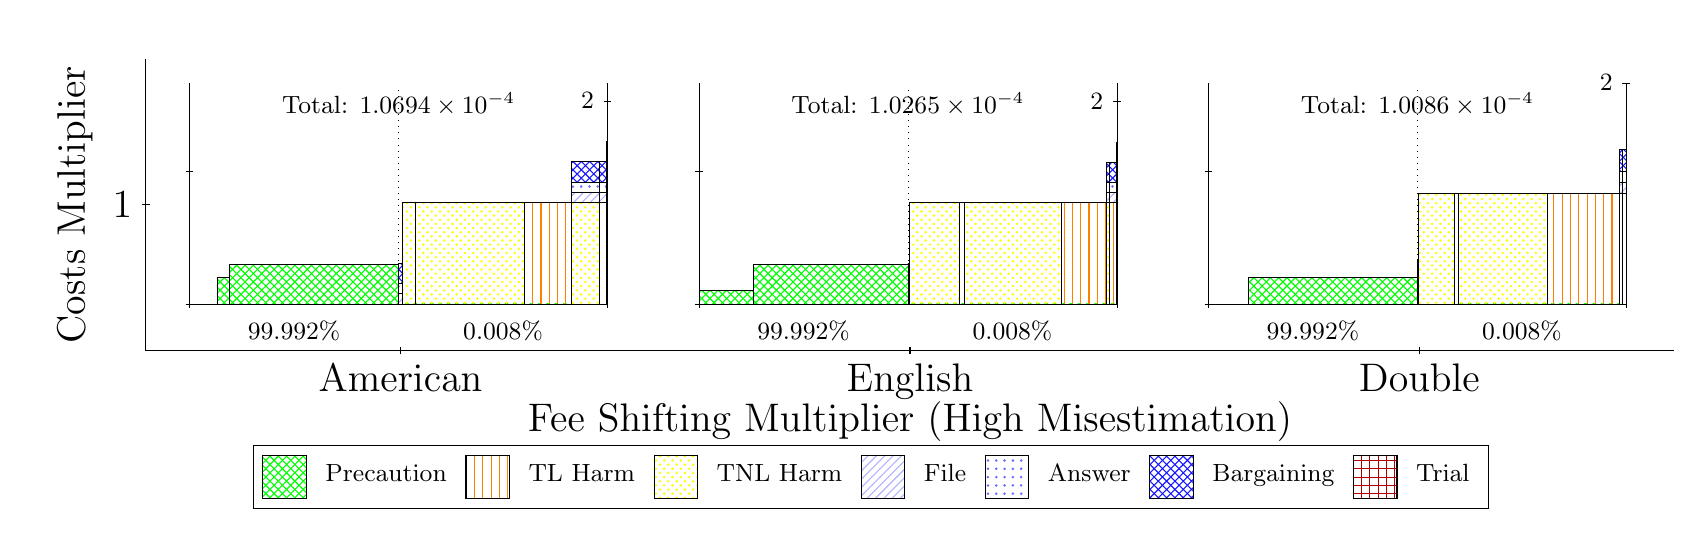
\begin{tikzpicture}
\clip(-0.5,-1.1) rectangle +(20.91,6.2);
\draw[black] (1,1) -- (1,4.7);
\node[rotate=90, fontscale=2, anchor=center] at (0.1, 2.85) {Costs Multiplier};
\draw[black] (0.95,2.85) -- (1.05,2.85);
\node[fontscale=2, anchor=east] at (0.95, 2.85) {1};

\draw[black] (1,1) -- (20.41,1);
\node[fontscale=2, anchor=center] at (10.705, 0.1) {Fee Shifting Multiplier (High Misestimation)};
\draw[black] (4.235,0.95) -- (4.235,1.05);
\node[fontscale=2, anchor=north] at (4.235, 0.95) {American};
\draw[black] (10.705,0.95) -- (10.705,1.05);
\node[fontscale=2, anchor=north] at (10.705, 0.95) {English};
\draw[black] (17.175,0.95) -- (17.175,1.05);
\node[fontscale=2, anchor=north] at (17.175, 0.95) {Double};


\draw[pattern=crosshatch, pattern color=green,draw=black,very thin] (1.9026,1.592) rectangle (2.0595,1.9276);
\draw[pattern=crosshatch, pattern color=green,draw=black,very thin] (2.0595,1.592) rectangle (4.21,2.0955);
\draw[pattern=north east lines, pattern color=blue!30,draw=black,very thin] (4.21,1.592) rectangle (4.2541,1.7209);
\draw[pattern=dots,  pattern color=blue!60,draw=black,very thin] (4.21,1.7209) rectangle (4.2541,1.8499);
\draw[pattern=crosshatch,      pattern color=blue!90,draw=black,very thin] (4.21,1.8499) rectangle (4.2541,2.1077);
\draw[pattern=north east lines, pattern color=blue!30,draw=black,very thin] (4.2541,1.592) rectangle (4.2552,1.7209);
\draw[pattern=dots,  pattern color=blue!60,draw=black,very thin] (4.2541,1.7209) rectangle (4.2552,1.8499);
\draw[pattern=crosshatch,      pattern color=blue!90,draw=black,very thin] (4.2541,1.8499) rectangle (4.2552,2.1077);
\draw[pattern=grid,            pattern color=red!70!black,draw=black,very thin] (4.2541,2.1077) rectangle (4.2552,2.3656);
\draw[pattern=crosshatch, pattern color=green,draw=black,very thin] (4.2552,1.592) rectangle (4.422,1.592);
\draw[pattern=crosshatch dots, pattern color=yellow,draw=black,very thin] (4.2552,1.592) rectangle (4.422,2.8814);
\draw[pattern=crosshatch, pattern color=green,draw=black,very thin] (4.422,1.592) rectangle (5.8086,1.592);
\draw[pattern=crosshatch dots, pattern color=yellow,draw=black,very thin] (4.422,1.592) rectangle (5.8086,2.8814);
\draw[pattern=crosshatch, pattern color=green,draw=black,very thin] (5.8086,1.592) rectangle (6.4039,1.592);
\draw[pattern=vertical lines, pattern color=orange,draw=black,very thin] (5.8086,1.592) rectangle (6.4039,2.8814);
\draw[pattern=crosshatch dots, pattern color=yellow,draw=black,very thin] (6.4039,1.592) rectangle (6.7535,2.8814);
\draw[pattern=north east lines, pattern color=blue!30,draw=black,very thin] (6.4039,2.8814) rectangle (6.7535,3.0103);
\draw[pattern=dots,  pattern color=blue!60,draw=black,very thin] (6.4039,3.0103) rectangle (6.7535,3.1392);
\draw[pattern=crosshatch,      pattern color=blue!90,draw=black,very thin] (6.4039,3.1392) rectangle (6.7535,3.3971);
\draw[pattern=vertical lines, pattern color=orange,draw=black,very thin] (6.7535,1.592) rectangle (6.8448,2.8814);
\draw[pattern=north east lines, pattern color=blue!30,draw=black,very thin] (6.7535,2.8814) rectangle (6.8448,3.0103);
\draw[pattern=dots,  pattern color=blue!60,draw=black,very thin] (6.7535,3.0103) rectangle (6.8448,3.1392);
\draw[pattern=crosshatch,      pattern color=blue!90,draw=black,very thin] (6.7535,3.1392) rectangle (6.8448,3.3971);
\draw[pattern=crosshatch, pattern color=green,draw=black,very thin] (6.8448,1.592) rectangle (6.8519,1.592);
\draw[pattern=crosshatch dots, pattern color=yellow,draw=black,very thin] (6.8448,1.592) rectangle (6.8519,2.8814);
\draw[pattern=north east lines, pattern color=blue!30,draw=black,very thin] (6.8448,2.8814) rectangle (6.8519,3.0103);
\draw[pattern=dots,  pattern color=blue!60,draw=black,very thin] (6.8448,3.0103) rectangle (6.8519,3.1393);
\draw[pattern=crosshatch,      pattern color=blue!90,draw=black,very thin] (6.8448,3.1393) rectangle (6.8519,3.3971);
\draw[pattern=crosshatch, pattern color=green,draw=black,very thin] (6.8519,1.592) rectangle (6.8523,1.592);
\draw[pattern=vertical lines, pattern color=orange,draw=black,very thin] (6.8519,1.592) rectangle (6.8523,2.8814);
\draw[pattern=north east lines, pattern color=blue!30,draw=black,very thin] (6.8519,2.8814) rectangle (6.8523,3.0103);
\draw[pattern=dots,  pattern color=blue!60,draw=black,very thin] (6.8519,3.0103) rectangle (6.8523,3.1393);
\draw[pattern=crosshatch,      pattern color=blue!90,draw=black,very thin] (6.8519,3.1393) rectangle (6.8523,3.3971);
\draw[pattern=crosshatch dots, pattern color=yellow,draw=black,very thin] (6.8523,1.592) rectangle (6.8531,2.8814);
\draw[pattern=north east lines, pattern color=blue!30,draw=black,very thin] (6.8523,2.8814) rectangle (6.8531,3.0103);
\draw[pattern=dots,  pattern color=blue!60,draw=black,very thin] (6.8523,3.0103) rectangle (6.8531,3.1392);
\draw[pattern=crosshatch,      pattern color=blue!90,draw=black,very thin] (6.8523,3.1392) rectangle (6.8531,3.3971);
\draw[pattern=grid,            pattern color=red!70!black,draw=black,very thin] (6.8523,3.3971) rectangle (6.8531,3.655);
\draw[pattern=vertical lines, pattern color=orange,draw=black,very thin] (6.8531,1.592) rectangle (6.863,2.8814);
\draw[pattern=north east lines, pattern color=blue!30,draw=black,very thin] (6.8531,2.8814) rectangle (6.863,3.0103);
\draw[pattern=dots,  pattern color=blue!60,draw=black,very thin] (6.8531,3.0103) rectangle (6.863,3.1392);
\draw[pattern=crosshatch,      pattern color=blue!90,draw=black,very thin] (6.8531,3.1392) rectangle (6.863,3.3971);
\draw[pattern=grid,            pattern color=red!70!black,draw=black,very thin] (6.8531,3.3971) rectangle (6.863,3.655);
\draw[pattern=crosshatch, pattern color=green,draw=black,very thin] (6.863,1.592) rectangle (6.8641,1.592);
\draw[pattern=crosshatch dots, pattern color=yellow,draw=black,very thin] (6.863,1.592) rectangle (6.8641,2.8814);
\draw[pattern=north east lines, pattern color=blue!30,draw=black,very thin] (6.863,2.8814) rectangle (6.8641,3.0103);
\draw[pattern=dots,  pattern color=blue!60,draw=black,very thin] (6.863,3.0103) rectangle (6.8641,3.1393);
\draw[pattern=crosshatch,      pattern color=blue!90,draw=black,very thin] (6.863,3.1393) rectangle (6.8641,3.3971);
\draw[pattern=grid,            pattern color=red!70!black,draw=black,very thin] (6.863,3.3971) rectangle (6.8641,3.655);
\draw[pattern=crosshatch, pattern color=green,draw=black,very thin] (6.8641,1.592) rectangle (6.8644,1.592);
\draw[pattern=vertical lines, pattern color=orange,draw=black,very thin] (6.8641,1.592) rectangle (6.8644,2.8814);
\draw[pattern=north east lines, pattern color=blue!30,draw=black,very thin] (6.8641,2.8814) rectangle (6.8644,3.0103);
\draw[pattern=dots,  pattern color=blue!60,draw=black,very thin] (6.8641,3.0103) rectangle (6.8644,3.1393);
\draw[pattern=crosshatch,      pattern color=blue!90,draw=black,very thin] (6.8641,3.1393) rectangle (6.8644,3.3971);
\draw[pattern=grid,            pattern color=red!70!black,draw=black,very thin] (6.8641,3.3971) rectangle (6.8644,3.655);
\node[font=\small,text=black,anchor=north] at (4.21, 4.4) {Total: $1.0694\times 10^{-4}$};
\draw[black,very thin] (1.5556,1.592) -- (1.5556,4.4);
\draw[black,very thin] (1.5056,1.592) -- (1.6056,1.592);
\node[font=\small,text=black, anchor=west] at (1.5056, 1.592) {};
\draw[black,very thin] (1.5056,3.2702) -- (1.6056,3.2702);
\node[font=\small,text=black, anchor=west] at (1.5056, 3.2702) {};

\draw[black,dotted,very thin] (4.21,1.6762) -- (4.21,4.3158);
\draw[black,very thin] (6.8644,1.592) -- (6.8644,4.4);
\draw[black,very thin] (6.8144,4.1707) -- (6.9144,4.1707);
\node[font=\small,text=black, anchor=east] at (6.8144, 4.1707) {\contour{white}{2}};

\draw[black,very thin] (1.5556,1.592) -- (6.8644,1.592);
\draw[black,very thin] (1.5556,1.542) -- (1.5556,1.642);
\node[font=\small,text=black, anchor=north] at (1.5556, 1.542) {};
\draw[black,very thin] (6.8644,1.542) -- (6.8644,1.642);
\node[font=\small,text=black, anchor=north] at (6.8644, 1.542) {};

\node[font=\small,text=black,anchor=south] at (2.8828, 0.992) {99.992\%};
\node[font=\small,text=black,anchor=south] at (5.5372, 0.992) {0.008\%};

\draw[pattern=crosshatch, pattern color=green,draw=black,very thin] (8.0256,1.592) rectangle (8.7203,1.7598);
\draw[pattern=crosshatch, pattern color=green,draw=black,very thin] (8.7203,1.592) rectangle (10.68,2.0955);
\draw[pattern=crosshatch, pattern color=green,draw=black,very thin] (10.68,1.592) rectangle (10.694,1.592);
\draw[pattern=north east lines, pattern color=blue!30,draw=black,very thin] (10.68,1.592) rectangle (10.694,1.7205);
\draw[pattern=dots,  pattern color=blue!60,draw=black,very thin] (10.68,1.7205) rectangle (10.694,1.8489);
\draw[pattern=crosshatch,      pattern color=blue!90,draw=black,very thin] (10.68,1.8489) rectangle (10.694,2.1059);
\draw[pattern=crosshatch, pattern color=green,draw=black,very thin] (10.694,1.592) rectangle (10.695,1.592);
\draw[pattern=north east lines, pattern color=blue!30,draw=black,very thin] (10.694,1.592) rectangle (10.695,1.7205);
\draw[pattern=dots,  pattern color=blue!60,draw=black,very thin] (10.694,1.7205) rectangle (10.695,1.8489);
\draw[pattern=crosshatch,      pattern color=blue!90,draw=black,very thin] (10.694,1.8489) rectangle (10.695,2.1059);
\draw[pattern=grid,            pattern color=red!70!black,draw=black,very thin] (10.694,2.1059) rectangle (10.695,2.3628);
\draw[pattern=crosshatch, pattern color=green,draw=black,very thin] (10.695,1.592) rectangle (11.329,1.592);
\draw[pattern=crosshatch dots, pattern color=yellow,draw=black,very thin] (10.695,1.592) rectangle (11.329,2.8767);
\draw[pattern=crosshatch, pattern color=green,draw=black,very thin] (11.329,1.592) rectangle (11.393,1.592);
\draw[pattern=vertical lines, pattern color=orange,draw=black,very thin] (11.329,1.592) rectangle (11.393,2.8767);
\draw[pattern=crosshatch, pattern color=green,draw=black,very thin] (11.393,1.592) rectangle (12.628,1.592);
\draw[pattern=crosshatch dots, pattern color=yellow,draw=black,very thin] (11.393,1.592) rectangle (12.628,2.8767);
\draw[pattern=crosshatch, pattern color=green,draw=black,very thin] (12.628,1.592) rectangle (13.203,1.592);
\draw[pattern=vertical lines, pattern color=orange,draw=black,very thin] (12.628,1.592) rectangle (13.203,2.8767);
\draw[pattern=crosshatch, pattern color=green,draw=black,very thin] (13.203,1.592) rectangle (13.24,1.592);
\draw[pattern=crosshatch dots, pattern color=yellow,draw=black,very thin] (13.203,1.592) rectangle (13.24,2.8767);
\draw[pattern=north east lines, pattern color=blue!30,draw=black,very thin] (13.203,2.8767) rectangle (13.24,3.0051);
\draw[pattern=dots,  pattern color=blue!60,draw=black,very thin] (13.203,3.0051) rectangle (13.24,3.1336);
\draw[pattern=crosshatch,      pattern color=blue!90,draw=black,very thin] (13.203,3.1336) rectangle (13.24,3.3905);
\draw[pattern=crosshatch, pattern color=green,draw=black,very thin] (13.24,1.592) rectangle (13.323,1.592);
\draw[pattern=vertical lines, pattern color=orange,draw=black,very thin] (13.24,1.592) rectangle (13.323,2.8767);
\draw[pattern=north east lines, pattern color=blue!30,draw=black,very thin] (13.24,2.8767) rectangle (13.323,3.0051);
\draw[pattern=dots,  pattern color=blue!60,draw=black,very thin] (13.24,3.0051) rectangle (13.323,3.1336);
\draw[pattern=crosshatch,      pattern color=blue!90,draw=black,very thin] (13.24,3.1336) rectangle (13.323,3.3905);
\draw[pattern=crosshatch, pattern color=green,draw=black,very thin] (13.323,1.592) rectangle (13.326,1.592);
\draw[pattern=crosshatch dots, pattern color=yellow,draw=black,very thin] (13.323,1.592) rectangle (13.326,2.8767);
\draw[pattern=north east lines, pattern color=blue!30,draw=black,very thin] (13.323,2.8767) rectangle (13.326,3.0051);
\draw[pattern=dots,  pattern color=blue!60,draw=black,very thin] (13.323,3.0051) rectangle (13.326,3.1336);
\draw[pattern=crosshatch,      pattern color=blue!90,draw=black,very thin] (13.323,3.1336) rectangle (13.326,3.3905);
\draw[pattern=grid,            pattern color=red!70!black,draw=black,very thin] (13.323,3.3905) rectangle (13.326,3.6475);
\draw[pattern=crosshatch, pattern color=green,draw=black,very thin] (13.326,1.592) rectangle (13.334,1.592);
\draw[pattern=vertical lines, pattern color=orange,draw=black,very thin] (13.326,1.592) rectangle (13.334,2.8767);
\draw[pattern=north east lines, pattern color=blue!30,draw=black,very thin] (13.326,2.8767) rectangle (13.334,3.0051);
\draw[pattern=dots,  pattern color=blue!60,draw=black,very thin] (13.326,3.0051) rectangle (13.334,3.1336);
\draw[pattern=crosshatch,      pattern color=blue!90,draw=black,very thin] (13.326,3.1336) rectangle (13.334,3.3905);
\draw[pattern=grid,            pattern color=red!70!black,draw=black,very thin] (13.326,3.3905) rectangle (13.334,3.6475);
\node[font=\small,text=black,anchor=north] at (10.68, 4.4) {Total: $1.0265\times 10^{-4}$};
\draw[black,very thin] (8.0256,1.592) -- (8.0256,4.4);
\draw[black,very thin] (7.9756,1.592) -- (8.0756,1.592);
\node[font=\small,text=black, anchor=west] at (7.9756, 1.592) {};
\draw[black,very thin] (7.9756,3.2702) -- (8.0756,3.2702);
\node[font=\small,text=black, anchor=west] at (7.9756, 3.2702) {};

\draw[black,dotted,very thin] (10.68,1.6762) -- (10.68,4.3158);
\draw[black,very thin] (13.334,1.592) -- (13.334,4.4);
\draw[black,very thin] (13.284,4.1613) -- (13.384,4.1613);
\node[font=\small,text=black, anchor=east] at (13.284, 4.1613) {\contour{white}{2}};

\draw[black,very thin] (8.0256,1.592) -- (13.334,1.592);
\draw[black,very thin] (8.0256,1.542) -- (8.0256,1.642);
\node[font=\small,text=black, anchor=north] at (8.0256, 1.542) {};
\draw[black,very thin] (13.334,1.542) -- (13.334,1.642);
\node[font=\small,text=black, anchor=north] at (13.334, 1.542) {};

\node[font=\small,text=black,anchor=south] at (9.3528, 0.992) {99.992\%};
\node[font=\small,text=black,anchor=south] at (12.007, 0.992) {0.008\%};

\draw[pattern=crosshatch, pattern color=green,draw=black,very thin] (15,1.592) rectangle (17.15,1.9276);
\draw[pattern=north east lines, pattern color=blue!30,draw=black,very thin] (17.15,1.592) rectangle (17.159,1.7324);
\draw[pattern=dots,  pattern color=blue!60,draw=black,very thin] (17.15,1.7324) rectangle (17.159,1.8728);
\draw[pattern=crosshatch,      pattern color=blue!90,draw=black,very thin] (17.15,1.8728) rectangle (17.159,2.1536);
\draw[pattern=crosshatch dots, pattern color=yellow,draw=black,very thin] (17.159,1.592) rectangle (17.612,2.996);
\draw[pattern=vertical lines, pattern color=orange,draw=black,very thin] (17.612,1.592) rectangle (17.671,2.996);
\draw[pattern=crosshatch, pattern color=green,draw=black,very thin] (17.671,1.592) rectangle (18.802,1.592);
\draw[pattern=crosshatch dots, pattern color=yellow,draw=black,very thin] (17.671,1.592) rectangle (18.802,2.996);
\draw[pattern=crosshatch, pattern color=green,draw=black,very thin] (18.802,1.592) rectangle (19.714,1.592);
\draw[pattern=vertical lines, pattern color=orange,draw=black,very thin] (18.802,1.592) rectangle (19.714,2.996);
\draw[pattern=crosshatch dots, pattern color=yellow,draw=black,very thin] (19.714,1.592) rectangle (19.752,2.996);
\draw[pattern=north east lines, pattern color=blue!30,draw=black,very thin] (19.714,2.996) rectangle (19.752,3.1364);
\draw[pattern=dots,  pattern color=blue!60,draw=black,very thin] (19.714,3.1364) rectangle (19.752,3.2768);
\draw[pattern=crosshatch,      pattern color=blue!90,draw=black,very thin] (19.714,3.2768) rectangle (19.752,3.5576);
\draw[pattern=vertical lines, pattern color=orange,draw=black,very thin] (19.752,1.592) rectangle (19.801,2.996);
\draw[pattern=north east lines, pattern color=blue!30,draw=black,very thin] (19.752,2.996) rectangle (19.801,3.1364);
\draw[pattern=dots,  pattern color=blue!60,draw=black,very thin] (19.752,3.1364) rectangle (19.801,3.2768);
\draw[pattern=crosshatch,      pattern color=blue!90,draw=black,very thin] (19.752,3.2768) rectangle (19.801,3.5576);
\draw[pattern=crosshatch dots, pattern color=yellow,draw=black,very thin] (19.801,1.592) rectangle (19.802,2.996);
\draw[pattern=north east lines, pattern color=blue!30,draw=black,very thin] (19.801,2.996) rectangle (19.802,3.1364);
\draw[pattern=dots,  pattern color=blue!60,draw=black,very thin] (19.801,3.1364) rectangle (19.802,3.2768);
\draw[pattern=crosshatch,      pattern color=blue!90,draw=black,very thin] (19.801,3.2768) rectangle (19.802,3.5576);
\draw[pattern=grid,            pattern color=red!70!black,draw=black,very thin] (19.801,3.5576) rectangle (19.802,3.8384);
\draw[pattern=vertical lines, pattern color=orange,draw=black,very thin] (19.802,1.592) rectangle (19.804,2.996);
\draw[pattern=north east lines, pattern color=blue!30,draw=black,very thin] (19.802,2.996) rectangle (19.804,3.1364);
\draw[pattern=dots,  pattern color=blue!60,draw=black,very thin] (19.802,3.1364) rectangle (19.804,3.2768);
\draw[pattern=crosshatch,      pattern color=blue!90,draw=black,very thin] (19.802,3.2768) rectangle (19.804,3.5576);
\draw[pattern=grid,            pattern color=red!70!black,draw=black,very thin] (19.802,3.5576) rectangle (19.804,3.8384);
\node[font=\small,text=black,anchor=north] at (17.15, 4.4) {Total: $1.0086\times 10^{-4}$};
\draw[black,very thin] (14.496,1.592) -- (14.496,4.4);
\draw[black,very thin] (14.446,1.592) -- (14.546,1.592);
\node[font=\small,text=black, anchor=west] at (14.446, 1.592) {};
\draw[black,very thin] (14.446,3.2702) -- (14.546,3.2702);
\node[font=\small,text=black, anchor=west] at (14.446, 3.2702) {};

\draw[black,dotted,very thin] (17.15,1.6762) -- (17.15,4.3158);
\draw[black,very thin] (19.804,1.592) -- (19.804,4.4);
\draw[black,very thin] (19.754,4.4) -- (19.854,4.4);
\node[font=\small,text=black, anchor=east] at (19.754, 4.4) {\contour{white}{2}};

\draw[black,very thin] (14.496,1.592) -- (19.804,1.592);
\draw[black,very thin] (14.496,1.542) -- (14.496,1.642);
\node[font=\small,text=black, anchor=north] at (14.496, 1.542) {};
\draw[black,very thin] (19.804,1.542) -- (19.804,1.642);
\node[font=\small,text=black, anchor=north] at (19.804, 1.542) {};

\node[font=\small,text=black,anchor=south] at (15.823, 0.992) {99.992\%};
\node[font=\small,text=black,anchor=south] at (18.477, 0.992) {0.008\%};

\coordinate (LegendAnchor) at (10.205000000000002,0);
\begin{scope}[align=center]
\matrix[scale=0.6,draw=black,below=0.2cm of LegendAnchor,nodes={draw},column sep=0.12cm]{
\node[rectangle,draw,minimum width=0.55cm,minimum height=0.55cm,pattern=crosshatch, pattern color=green]{}; &
        \node[draw=none,font=\small]{Precaution}; &
\node[rectangle,draw,minimum width=0.55cm,minimum height=0.55cm,pattern=vertical lines, pattern color=orange]{}; &
        \node[draw=none,font=\small]{TL Harm}; &
\node[rectangle,draw,minimum width=0.55cm,minimum height=0.55cm,pattern=crosshatch dots, pattern color=yellow]{}; &
        \node[draw=none,font=\small]{TNL Harm}; &
\node[rectangle,draw,minimum width=0.55cm,minimum height=0.55cm,pattern=north east lines, pattern color=blue!30]{}; &
        \node[draw=none,font=\small]{File}; &
\node[rectangle,draw,minimum width=0.55cm,minimum height=0.55cm,pattern=dots, pattern color=blue!60]{}; &
        \node[draw=none,font=\small]{Answer}; &
\node[rectangle,draw,minimum width=0.55cm,minimum height=0.55cm,pattern=crosshatch, pattern color=blue!90]{}; &
        \node[draw=none,font=\small]{Bargaining}; &
\node[rectangle,draw,minimum width=0.55cm,minimum height=0.55cm,pattern=grid, pattern color=red!70!black]{}; &
        \node[draw=none,font=\small]{Trial}; \\
};\end{scope}

\end{tikzpicture}
\end{document}